
\subsection{Smaller Minimum Allocation Size}
\label{sec:future-work:lilliput}

The smallest possible unit of allocation inside ZGC is at the time or writing 16 bytes. This limit is due to the fact that object headers in Java are 16 bytes large, or 128 bits. However, work is currently in progress to reduce the size of the object header down to 64 bits or less through project Lilliput~\cite{lilliput}. Since Lilliput is still work in progress, the smaller allocation size of 8 bytes has not been supported in the general nor optimized version of the allocator.


Blocks that are smaller than 16 bytes require very little information on their particular size, which goes against using 8 bytes for storing size information, as detailed in Section~\ref{sec:adaptations_impl:0-byte-header}. Furthermore, as discussed in Section~\ref{sec:tlsf} regarding the design of TLSF and continuing in Section~\ref{sec:adaptations:architectural-considerations} on architectural adjustments, there is now an extra bit available for storing metadata inside block headers when aligning allocations to 8 bytes instead of 4 bytes. One might use this third metadata bit as a binary property to indicate whether a block is the smallest possible size, 8 bytes, or not. If the bit is set, the size field in the block header can be replaced with the next and prev pointers, making it possible to store all metadata about the block inside 8 bytes.

% TODO: Fix image
%\begin{figure}[H]
    %\centering
    %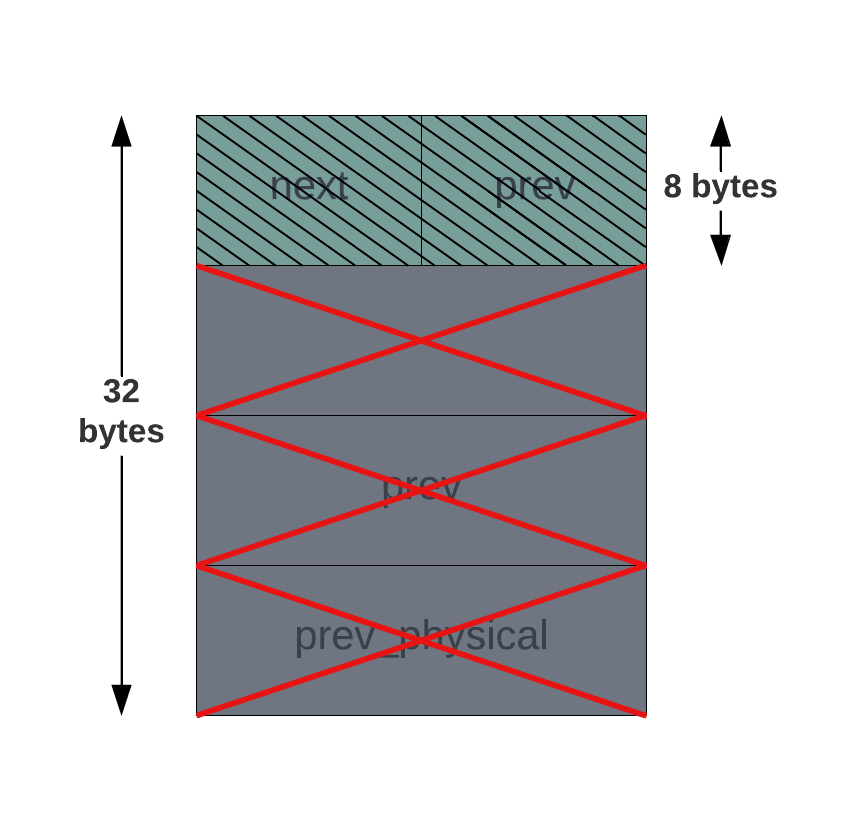
\includegraphics[width=0.5\textwidth]{figures/blockheader_lilliput.png}
    %\caption{Illustration of what the block header could contain after adjustments for Lilliput.}
    %\label{fig:lilliput_block_header}
%\end{figure}

%%% Local Variables:
%%% mode: latex
%%% TeX-master: "main"
%%% End:
